\documentclass[draft]{hcmut-report}
\usepackage{codespace}
\usepackage{amssymb}
% Sub-preambles
% https://github.com/MartinScharrer/standalone
% use to create href
\usepackage{hyperref}
\usepackage{minted} % for minted code
% Encodings
\usepackage{gensymb,textcomp}

% Better tables
% Wide tables go to https://tex.stackexchange.com/q/332902
\usepackage{array,multicol,multirow,siunitx,tabularx}
\usepackage{blindtext}
% Better enum
\usepackage{enumitem}

% Graphics
\usepackage{caption,float}

% Allow setting >max< width of figure
% 'export' allows adjustbox keys in \includegraphics
% For demonstration purposes, remove in production
\usepackage[export]{adjustbox}

% For demonstration purposes, remove in production
\usepackage{mwe}

% Configurations
\ocoursename{Course name h}
\oreporttype{Report type h}
\title{Report title h}
\oadvisor{Advisor h}
\newcounter{memberrowno}
\setcounter{memberrowno}{0}

% Custom commands
\newcommand*\mean[1]{\bar{#1}}

\begin{document}
\coverpage%

% ============ Member list and Workload ============ (TURNED OFF)
% \section*{Member list \& Workload}
% \begin{center}
%   \begin{tabular}{>{\stepcounter{memberrowno}\thememberrowno}llcc}
%     \toprule
%     \multicolumn{1}{c}{\textbf{No.}} & \textbf{Full name} & \textbf{Student ID} & \textbf{Contribution} \\
%     \midrule
%                                      & h                  & xxxxxxx             & 100\%                       \\
%                                      & h                  & xxxxxxx             & 100\%                       \\
%     \bottomrule
%   \end{tabular}
% \end{center}

\newpage
\tableofcontents
\newpage

% ============ Viet Tung reply ============ (TURNED OFF)
% \section{Preface}
\blindtext[5]
\newpage
% \section{Data analysis}

\subsection{Data descrition}
\subsubsection{Describing the data.}
For the first part of our project, we need to select a suitable dataset for us to analyze, as we are computer science students, we have decided to select a CPU data set, the data of which can be found \href{https://www.kaggle.com/datasets/iliassekkaf/computerparts?select=Intel_CPUs.csv}{here}:

The structure of our data set includes a total of 45 columns and 2283 instances.

Our data attribute:
\
\checkmark means we should ye analyze.
\begin{itemize}
    \item Product\_Collection: tell us which type of series the core belongs to.
    \item Vertical\_Segment: show what kind of system the CPU was designed for (embedded, mobile, desktop, or sever) \checkmark (could draw box plot for fun).
    \item Processor\_Number	: process ID.
    \item Status: show the status of the CPU (announce, launched, end of life, end of support) \checkmark
    \item Launch\_Date: The date the product was first introduced. \checkmark
    \item Lithography: refers to the semiconductor technology used to manufacture an integrated circuit, and is reported in nanometers (nm), indicative of the size of features built on the semiconductor. (the smaller the better, the smaller one also produces less heat). \checkmark
    \item Recommended\_Customer\_Price: recommended customer price. \checkmark
    \item nb\_of\_Cores: total cores in a proccessor. \checkmark
    \item nb\_of\_Threads: total cores in a processor. \checkmark
    \item Processor\_Base\_Frequency: Describes the rate at which the processor's transistors open and close. (number of cycle per amount of time the higher the better) \checkmark
    \item Max\_Turbo\_Frequency: The maximum single core frequency at which the processor is capable of operating using Intel® Turbo Boost Technology. 
    \item Cache: CPU Cache is an area of fast memory located on the processor. 
    \item Bus\_Speed: refers to how much data can move across the bus simultaneously.
    \item TDP(thermal design power): Represents the average power, in watts, the processor dissipates when operating at Base Frequency with all cores. (what NK is actually looking for) \checkmark
    \item Embedded\_Options\_Available: is it allow to be embedded system
    \item Conflict\_Free: Defined by the U.S. Securities and Exchange Commission rules to mean products that do not contain conflict minerals (tin, tantalum, tungsten)
    \item Max\_Memory\_Size: The maximum memory capacity supported by the processor. \checkmark
    \item Memory\_Types: Single Channel, Dual Channel, Triple Channel, and Flex Mode.The maximum memory capacity supported by the processor.
    \item Max\_nb\_of\_Memory\_Channels: The number of memory channels refers to the bandwidth operation for real world application.
    \item Max\_Memory\_Bandwidth: The maximum rate at which data can be read from or stored into a semiconductor memory by the processor (in GB/s). \checkmark
    \item ECC\_Memory\_Supported: ECC memory is a type of system memory that can detect and correct common kinds of internal data corruption.
    \item Processor\_Graphics: integrated graphics processing unit (GPU) that is built into some of Intel's processors.
    \item Graphics\_Base\_Frequency: The rated/guaranteed graphics render clock frequency in MHz.
    \item Graphics\_Max\_Dynamic\_Frequency: The maximum opportunistic graphics render clock frequency (in MHz) that can be supported using Intel HD Graphics with Frequency feature.
    \item Graphics\_Video\_Max\_Memory: The maximum amount of memory accessible to processor graphics. Processor graphics operates on the same physical memory as the CPU (subject to OS, driver, and other system limitations).
    \item Graphics\_Output: Graphics Output defines the interfaces available to communicate with display devices.
    \item Support\_4k: indicates the product's support of 4K
    \item Max\_Resolution\_HDMI: the maximum resolution supported by the processor via the HDMI interface (24bits per pixel \&amp; 60Hz). System or device display resolution is dependent on multiple system design factors; actual resolution may be lower on your system.
    \item Max\_Resolution\_DP: The maximum resolution supported by the processor via the DP interface (24bits per pixel \&amp; 60Hz). System or device display resolution is dependent on multiple system design factors.
    \item Max\_Resolution\_eDP\_Integrated\_Flat\_Panel	
    \item DirectX\_Support: Indicates support for a specific version of DirectX, a Microsoft collection of APIs for handling multimedia compute tasks.
    \item OpenGL\_Support: Indicates support for OpenGL, a cross-language, multi-platform API for rendering 2D and 3D vector graphics. (ye this is also NULL)
    \item PCI\_Express\_Revision: The PCIe version supported by the processor. 
    \item PCI\_Express\_Configurations\_: The available PCIe lane configurations that can be used to link the PCH PCIe lanes to PCIe devices.
    \item T : The maximum temperature allowed on the chip. \checkmark
    \item Max\_nb\_of\_PCI\_Express\_Lanes: maximum number of PCI Express Lanes that are supported.
    \item Intel\_Hyper\_Threading\_Technology\_: Delivers two processing threads per physical core. Highly threaded applications can get more work done in parallel, completing tasks sooner.
    \item Intel\_Virtualization\_Technology\_VTx\_: Allows one hardware platform to function as multiple “virtual” platforms. It offers improved manageability by limiting downtime and maintaining productivity by isolating computing activities into separate partitions.
    \item Intel\_64\_: Delivers 64-bit computing on server, workstation, desktop and mobile platforms when combined with supporting software. Intel 64 architecture improves performance by allowing systems to address more than 4 GB of both virtual and physical memory.
    \item Instruction\_Set: Which instrution set the CPU use.
    \item Instruction\_Set\_Extensions :  Instruction set extension
    \item Idle\_States: Used to save power when the processor is idle.
    \item Thermal\_Monitoring\_Technologies: Protects the processor package and the system from thermal failure through several thermal management features.	
    \item Secure\_Key: The CPU is supported with secure key or not.
    \item Execute\_Disable\_Bit: Hardware-based security feature that can reduce exposure to viruses and malicious code attacks.
\end{itemize}




\subsection{Data Preprocessing}
As we primarily only focus on analyzing \emph{some thing fill later}. We will only keep a couple of feature, that include: Vertical\_Segment, Status, Launch\_Date, Lithography, Recommended\_Customer\_Price, nb\_of\_Cores, nb\_of\_Threads, Processor\_Base\_Frequency, TDP, Max\_Memory\_Bandwidth, T.

As the data has a lot of unnecessary \_ in the code so we will rename it for more convenient coding.

Will insert it after we have agree on the feature.



% \section{Conclusion}
\blindtext[5]

% ============ Template ============ (TURNED OFF)
%\section{Better tables}
The recommended way is by using the booktabs package and drop all vertical rules.

Tabularx is simply tabular but with X environment, meaning that it will try to use all of \mintinline{latex}{\linewidth}.

\begin{center}
  \begin{tabularx}{\linewidth}{l*{2}{X}}
    \toprule
         & OOP & FP \\
    \cmidrule(lr){2-3}
    Pros &     &    \\
         &     &    \\
         &     &    \\
    \midrule
    Cons &     &    \\
         &     &    \\
         &     &    \\
    \bottomrule
  \end{tabularx}
\end{center}

More information can be found at \url{https://latex-tutorial.com/tables-in-latex/}.

%\section{Better enumerator}
Normal enumerator gets the job done, but what if you want custom numbering?
This implementation allows custom labeling, either by pre-defined rules or in-place.

\begin{enumerate}[label={\alph*.yeah}]
  \item First item
  \item Second item
  \item[custom] Third item
\end{enumerate}

%\section{Codeblocks}
There are several ways to embed code in a \LaTeX{} file.
Here are inline code, embedded codeblock, and external import.

\begin{itemize}
  \item External import

  \inputcode[highlightlines={1,10-13}]{Python}{code/example.py}

  \item With custom line range

  \inputcode[firstline=10,lastline=13]{Python}{code/example.py}

  \item Embedded

  \begin{code}{Python}
  class iostream:
      def __lshift__(self, other):
          print(other, end='')
          return self

      def __repr__(self):
          return ''
  \end{code}

  \item Inline

  \mintinline{Python}{print('Hello, world!')}
\end{itemize}

You can also define your custom inline as \url{https://tex.stackexchange.com/a/148479}.

This is one way to input algorithms.

\begin{algorithm}[H]
  \caption{QL algorithm}
  Initialize \(Q\)-table values \((Q(s, a))\) arbitrarily\;
  Initialize a state \((s_t)\)\;
  Repeat Steps~\ref{alg:step_4} to~\ref{alg:step_6} until learning period ends\;
  Choose an action \((a_t)\) for the current state \((s_t)\) using an exploratory policy\; \nllabel{alg:step_4}
  Take action \((a_t)\) and observe the new state \((s_t + 1)\) and reward \((r_t + 1)\)\;
  Update \(Q\)-value\; \nllabel{alg:step_6}
\end{algorithm}

%\section{Figures with flexible width}

\hrule % to see \linewidth

\includegraphics[max width=0.9\linewidth]{example-image-1x1}

\includegraphics[scale=0.7]{example-image-a4}

With \mintinline{latex}{\adjincludegraphics} (or \mintinline{latex}{\adjustimage}) you can also use the original width as \mintinline{latex}{\width}:

\adjincludegraphics[width=\ifdim \width > \linewidth \linewidth \else \width \fi]{example-image}


% ============ MAIN ============
% We will include official *.tex files here.
%
%   ABSTRACT
%
%   Total summary of our report.
%   Should include the following information
%       1.  [background] : Briefly introduce the topic, why the report is 
%           relevant to statistics
%       2.  [objectives] : What do we want , what are the aims?
%       3.  [statistical methods] : 
%       4.  [results]
%       5.  [conclusion]
%   
%   Should be written AFTER finishing the report
\clearpage
\section{Abstract}
%
%   BACKGROUND
%
%   Introduce external and additional knowledge (the methods we did not learn)
%   Le Hieu did present some weird stuff in this section (also called Theory Basis)
\clearpage
\section{Background}
\subsection{ANOVA.}
Analysis of variance (ANOVA) is a statistical method used to test for differences among two or more population means by analyzing the variances of samples taken from the populations.
\subsubsection{One way ANOVA.}
For one way ANOVA, we would like to anylyse the effect of a single factors with multiple level on a samples.

For each observation under the treatment $i$ under the $j$ observation called $y_{ij}$ we have the linear combination:

\[y_{ij} = \mu + \tau_i + \epsilon_{ij} 
\begin{cases}
    i = 1,2,...,a.\\
    j = 1,2,...,n.
\end{cases}
\]
Where:
\begin{itemize}
    \item $\mu$ is the overall mean.
    \item $\tau_i$ is the effect of the $i$th treatment effect.
    \item $\epsilon_{ij}$ is a random component error.
\end{itemize}
We could rewritten the model as.

\[y_{ij} = \mu_i + \epsilon_{ij} 
\begin{cases}
    i = 1,2,...,a.\\
    j = 1,2,...,n.
\end{cases}
\]
Where:
\begin{itemize}
    \item $\mu_i$ =  $\mu + \tau_i$
    \item $\tau_i$ is the effect of the $i$th treatment effect.
    \item $\epsilon_{ij}$ is a random component error.
\end{itemize}

if we assume that the errors $\epsilon_{ij}$ are normally and independently distributed with mean 0 and variance $\sigma^2$. Each treatment can be treated as a normal population with the mean of $\mu_i$ and variance $\sigma^2$.

So to perform a one way ANOVA the data will need to fufill the following assumption:
\begin{enumerate}
    \item Normality: The populations have distributions that are approximately normal.
    \item   : The populations have the same variance
    \item Independent: the data is random and independent.
\end{enumerate}
However the Normality and Homogeneity of variance are only loose requirement as the method still well despite failing these assumptionStatistician George E. P. Box.
However we will also use the Kruskal - Wallis test for anything that do not sastify the assumption.
We want to test the Null hypothesis:
\[
\begin{cases}
    H_0: \mu_1 = \mu_2 = ... = \mu_n \\
    H_1: \text{two mean are different}
\end{cases}
\]
Total sum of squares:
\[ SS_T = \sum_{i = 1}^{a} \sum_{j = 1}^{n} (y_{ij} - \bar{y})^2\]
\[ SS_T = n\sum_{i=1}^{a}(\bar{y_i}-\bar{y})^2 + \sum_{i=1}^{a}\sum_{j=1}^{n}(y_{ij}-\bar{y_i})^2\]
or
\[ SS_T = SS_{Treatment}+SS_{Error}\]
where degree of freedom is:
\[df(SS_T) = N - 1 \quad df(SS_{Treatment}) = a - 1 \quad df(SS_{Error}) = N - a \]
Mean square for treatments: 
\[MS_{Treatment} = SS_{Treatment} / df(SS_{Treatment})\]
\[MS_{Treatment} = SS_{Treatment} / (a - 1)\]
Mean square for error: 
\[MS_{Error} = SS_{Treatment} / df(SS_{Error})\]
\[MS_{Error} = SS_{Treatment} / (N - a)\]   
F test statistic: 
\[F_0 = \frac{MS_{Treatment}}{MS_{Error}}\]
If \[F_0 > F_{\alpha , a-1,a(n-1)}\]

\subsection{Two way ANOVA.}
similarly to one way, two way ANOVA is also a statistical method used to test for differences among two or more population means by analyzing the variances of samples taken from the populations. The difference here is that two way ANOVA used two factors for the test.

% We also have to the linear combination for each observation as followed:
% \[y_{ij} = \mu + \alpha_i + \beta_j +\gamma_{ij} +\epsilon_{ij}\]
% Where  
% \begin{itemize}
%     \item $\mu$ is the overall mean.
%     \item $\alpha_i$ is the additive main effect of the $i$th treatment effect.
%     \item $\beta_i$ is the additive main effect of the $j$th treatment effect.
%     \item $
%     \item $\epsilon_{ij}$ is a random component error.
% \end{itemize}
\subsection{Kruskal - Wallis test}
Kruskal - Wallis test which uses ranks of data from three or more independent simple random samples to test the null hypothesis that the samplees come from populations with the same median.
The Kruskal-Wallis test for equal medians does not require normal distributions, so it is a distribution-free or non parametric test. 
In applying the Kruskal - Wallis test we need to compute the test statistic H.
\[H = \frac{12}{N(N+1)*\sum_{i=1}^{k}\frac{R_i^2}{n_i}-3(N+1)}\]
Where:

\begin{itemize}
    \item $N$ is the number of values from all combined samples.
    \item $R_i$ is the sum of ranks from a paricular sample, and $n_i$ is the number of values from the corresponding rank sum.
    \item $n_i$ is the number of values from the corresponding rank sum.
\end{itemize}

\subsection{Levene test}
Levene's test is used to test if k samples have equal variance.In this assignment, we will use it as the primary tool for testing the Homogeneity of variance.

Given a variable Y with sample of sizeN divided into k subgroupsm where $N_i$ is the sample size of the $i$th subgroup, the Levene test is defined as:
\[
\begin{cases}
    H_0: \sigma_1^2 = \sigma_2^2 =...=\sigma_k^2
    H_1: there are at least one pair with unequal variance.
\end{cases}
\]
\[W = \frac{(N-K)}{(k-1)}\frac{\sum_{i=1}^{k}N_i(\bar{Z_i}-\bar{Z})^2}{\sum_{i=1}^{j}\sum_{j=1}^{N_i}(Z_{ij}-\bar{Z_i})^2}\]
where $Z_{ij}$ cahn have one of these following definitions:

\begin{itemize}
    \item $Z_{ij} = Y_{iJ} - \bar{Y_i}$ where $\bar{Y_i}$ is the mean  of the $i$th subgroup.
    \item $Z_{ij} = Y_{iJ} - \tilde{Y_i}$ where $\tilde{Y_i}$ is the median of the $i$th subgroup.
    \item $Z_{ij} = Y_{iJ} - \bar{Y_i}^{'}$ where $\bar{Y_i}^{'}$ is the trimmed mean of the $i$th subgroup.
\end{itemize}

The three choice for detemining $Z_{ij}$ determine the robustness and power of Levene's test. We will choose choice where $\tilde{Y_i}$ is the median as it is the default choice of LeveneTest in R

\subsection{Shapiro-Wilk test}
The Shapiro-Wilk test, calculates a W statistic that tests whether a random sample, $x_1$, $x_2$, ..., $x_n$ come from a normal distribution. 
The W statistic is calculated as:
\[W = \frac{(\sum_{i=1}^{n}a_ix_{(i)})^2}{\sum_{i=1}^{n}(x_i-\bar{x})^2}\]
where:
\begin{itemize}
    \item $x_{(i)}are the ordered sample values$
    \item $a_i$ are the constant generated from the means, variance and covariance of the order of a sample of size n from a normal distribution.
    \item $\bar{x}$ is the sample mean
\end{itemize}
We would like to use this test to test the Null hypothesis:
\[
\begin{cases}
    H_0: The population is normally distributed
    H_1: the population is not normally distributed
\end{cases}
\]
if the p-value is less than $\alpha$ then we can reject the null hypothesis this test and consider our data to not be Normally distributed.
\subsection{Post hoc test}
\subsubsection{TUKEY HSD test}

\subsubsection{Dunn test}




%
%   Data description
%       - Importing data
%       - Data preprocessing
%       - Data cleaning
%   
\clearpage
\section{Data description}









\subsection{Overview of the dataset}

Write something about the dataset, because no one will understand what a chip is 
if we don't elaborate them.

Some parts from Importing data section could be brought to here.










\subsection{Importing data}
For the first part of our project, we need to select a suitable dataset for us to analyze, as we are computer science students, we have decided to select a CPU data set, the data of which can be found \href{https://www.kaggle.com/datasets/iliassekkaf/computerparts?select=Intel_CPUs.csv}{here}:
\\
The data give us information about 2283 CPU and 45 of their attribute which include:
\\
\begin{itemize}
    \item Product\_Collection: tell us which type of series the core belongs to.
    \item Vertical\_Segment: show what kind of system the CPU was designed for (embedded, mobile, desktop, or sever).
    \item Processor\_Number	: process ID.
    \item Status: show the status of the CPU (announce, launched, end of life, end of support).
    \item Launch\_Date: The date the product was first introduced. 
    \item Lithography: refers to the semiconductor technology used to manufacture an integrated circuit, and is reported in nanometers (nm), indicative of the size of attributes built on the semiconductor. 
    \item Recommended\_Customer\_Price: recommended customer price. 
    \item nb\_of\_Cores: total number of cores in a proccessor. 
    \item nb\_of\_Threads: total number of thread in a processor. 
    \item Processor\_Base\_Frequency: Describes the rate at which the processor's transistors open and close.
    \item Max\_Turbo\_Frequency: The maximum single core frequency at which the processor is capable of operating using Intel® Turbo Boost Technology. 
    \item Cache: CPU Cache is an area of fast memory located on the processor. 
    \item Bus\_Speed: refers to how much data can move across the bus simultaneously.
    \item TDP(thermal design power): Represents the average power, in watts, the processor dissipates when operating at Base Frequency with all cores. 
    \item Embedded\_Options\_Available: is it allow to be embedded system
    \item Conflict\_Free: Defined by the U.S. Securities and Exchange Commission rules to mean products that do not contain conflict minerals (tin, tantalum, tungsten).
    \item Max\_Memory\_Size: The maximum memory capacity supported by the processor. 
    \item Memory\_Types: Single Channel, Dual Channel, Triple Channel, and Flex Mode.The maximum memory capacity supported by the processor.
    \item Max\_nb\_of\_Memory\_Channels: The number of memory channels refers to the bandwidth operation for real world application.
    \item Max\_Memory\_Bandwidth: The maximum rate at which data can be read from or stored into a semiconductor memory by the processor (in GB/s). 
    \item ECC\_Memory\_Supported: ECC memory is a type of system memory that can detect and correct common kinds of internal data corruption.
    \item Processor\_Graphics: integrated graphics processing unit (GPU) that is built into some of Intel's processors.
    \item Graphics\_Base\_Frequency: The rated/guaranteed graphics render clock frequency in MHz.
    \item Graphics\_Max\_Dynamic\_Frequency: The maximum opportunistic graphics render clock frequency (in MHz) that can be supported using Intel HD Graphics with Frequency attribute.
    \item Graphics\_Video\_Max\_Memory: The maximum amount of memory accessible to processor graphics. Processor graphics operates on the same physical memory as the CPU (subject to OS, driver, and other system limitations).
    \item Graphics\_Output: Graphics Output defines the interfaces available to communicate with display devices.
    \item Support\_4k: indicates the product's support of 4K
    \item Max\_Resolution\_HDMI: the maximum resolution supported by the processor via the HDMI interface (24bits per pixel \&amp; 60Hz). System or device display resolution is dependent on multiple system design factors; actual resolution may be lower on your system.
    \item Max\_Resolution\_DP: The maximum resolution supported by the processor via the DP interface (24bits per pixel \&amp; 60Hz). System or device display resolution is dependent on multiple system design factors.
    \item Max\_Resolution\_eDP\_Integrated\_Flat\_Panel	
    \item DirectX\_Support: Indicates support for a specific version of DirectX, a Microsoft collection of APIs for handling multimedia compute tasks.
    \item OpenGL\_Support: Indicates support for OpenGL, a cross-language, multi-platform API for rendering 2D and 3D vector graphics. 
    \item PCI\_Express\_Revision: The PCIe version supported by the processor. 
    \item PCI\_Express\_Configurations\_: The available PCIe lane configurations that can be used to link the PCH PCIe lanes to PCIe devices.
    \item T : The maximum temperature allowed on the chip.
    \item Max\_nb\_of\_PCI\_Express\_Lanes: maximum number of PCI Express Lanes that are supported.
    \item Intel\_Hyper\_Threading\_Technology\_: Delivers two processing threads per physical core. Highly threaded applications can get more work done in parallel, completing tasks sooner.
    \item Intel\_Virtualization\_Technology\_VTx\_: Allows one hardware platform to function as multiple “virtual” platforms. It offers improved manageability by limiting downtime and maintaining productivity by isolating computing activities into separate partitions.
    \item Intel\_64\_: Delivers 64-bit computing on server, workstation, desktop and mobile platforms when combined with supporting software. Intel 64 architecture improves performance by allowing systems to address more than 4 GB of both virtual and physical memory.
    \item Instruction\_Set: Which instrution set the CPU use.
    \item Instruction\_Set\_Extensions :  Instruction set extension
    \item Idle\_States: Used to save power when the processor is idle.
    \item Thermal\_Monitoring\_Technologies: Protects the processor package and the system from thermal failure through several thermal management attributes.	
    \item Secure\_Key: The CPU is supported with secure key or not.
    \item Execute\_Disable\_Bit: Hardware-based security attribute that can reduce exposure to viruses and malicious code attacks.
\end{itemize}

For coding the data, our team use a wide range of package which include 
\begin{itemize}
    \item \verb|rio|.
    \item \verb|ggplot2|.
    \item \verb|zoo|
\end{itemize}

Two primary packages used in this process are:

\begin{itemize}
    \item \verb|rio| : for intuitive I/O code.
    With this package, import and export dataset is easier and safer. It could 
    also handle multiple file formats, so that we do not have to
    change the command each time we change the file format.

    \item \verb|zoo| : for year-quarter format.
    In our data, the \verb|Launch date| is in non-standard format, and difficult to be operated on. This package helps to transform
    into standard year-quarter format, and provides useful operations, such as plotting and taking difference on these formats.

\end{itemize}

\inputcode[firstline=21,lastline=25]{R}{rcode/cleaning.r}

for importing in the code, we use the function \mintinline{R}{import()} from rio to import our data set.

\inputcode[firstline=6,lastline=9]{R}{rcode/importing.r}

MAY NEN NOI GI DO THEM, VI CAI NAY TAO CHUA VIET XONG!!!!

Viet tung do this.

You should describe how the attributes are chosen, why it is chosen, and stuff...

NK merge this preprocessing section with this section.
\subsection{Data preprocessing}

After examining the code, as we only want to focus on the performance and trend of the cpu designing, as there are many unesscessary such as Product\_Collection and Processor\_Number which only tell us about series of cpu they are from, some give only information about cpu hardware support, and some attribute which also has a lot of \mintinline{R}{NA} values which make it hard to anylyze the data.So our team has decided to cut back some attribute and use only a couple of them, that inlcude:

\textbf{Need}: Vertical\_Segment, Status, Launch\_Date, Lithography, Recommended\_Customer\_Price, nb\_of\_Cores, nb\_of\_Threads, Processor\_Base\_Frequency, TDP, Max\_Memory\_Bandwidth, T.

The reason for the choice of these attribute is that they are all give us a lot of information about the performance and effiecency. They are also often the most important factors in measuring the performance of each cpu.

\inputcode[firstline = 10,lastline=15]{R}{rcode/importing.r}

\textbf{Changing labels}

The original labels are very long and descriptive, we might not want that such level of details during coding. Therefore, the labels are suppressed
into small, compact abbreviations. The mapping of each label is summarized in the below table:

\begin{center}
    \begin{tabularx}{\linewidth}{l*{2}{X}}
        \toprule
        \verb|Vertical segment -> market| & \verb|Status -> status|  & \verb|Launch date -> ldate|      \\
        \verb|Lithography -> litho| & \verb|Recommended price -> rprice|  & \verb|Num. cores -> ncore|  \\
        \verb|Base frequency -> bfreq| & \verb|TDP -> tdp|   & \verb|Memory bandwidth -> memband|       \\
        \verb|T -> temp| & &                                                                            \\
        \bottomrule
    \end{tabularx}
\end{center}

\inputcode[firstline=16,lastline=20]{R}{rcode/importing.r}









\subsection{Data cleaning}
After choosing the approriate attributes, we now have the subset of the original raw dataset. 
However, since the values vary in types (such as string, non-standard year-quarter format and numeric-string),
we might want transform them into reproducible types, so that the analysis later on is easier, homogeneous and accurate.

Note that this cleaning process \textbf{does not} remove the \mintinline{R}{NA} values, unless necessary. The reason is that, 
in one instance, there might be important values that should not be eliminated. Under different scopes of study, we can not treat 
instances with \mintinline{R}{NA} as an invalid datum for all scopes. In later sections, when we focus on a specific pattern of the data, only by then
that the data will have a tailored \mintinline{R}{NA} cleaning, and we will not, by chance, loose any important instance.

This process took \verb|/rcode/cpu-short.csv| from the importing procedure above as an input, and produce \verb|/rcode/cpu-clean.csv| as
an output.

\begin{figure}[h!]
    \centering
    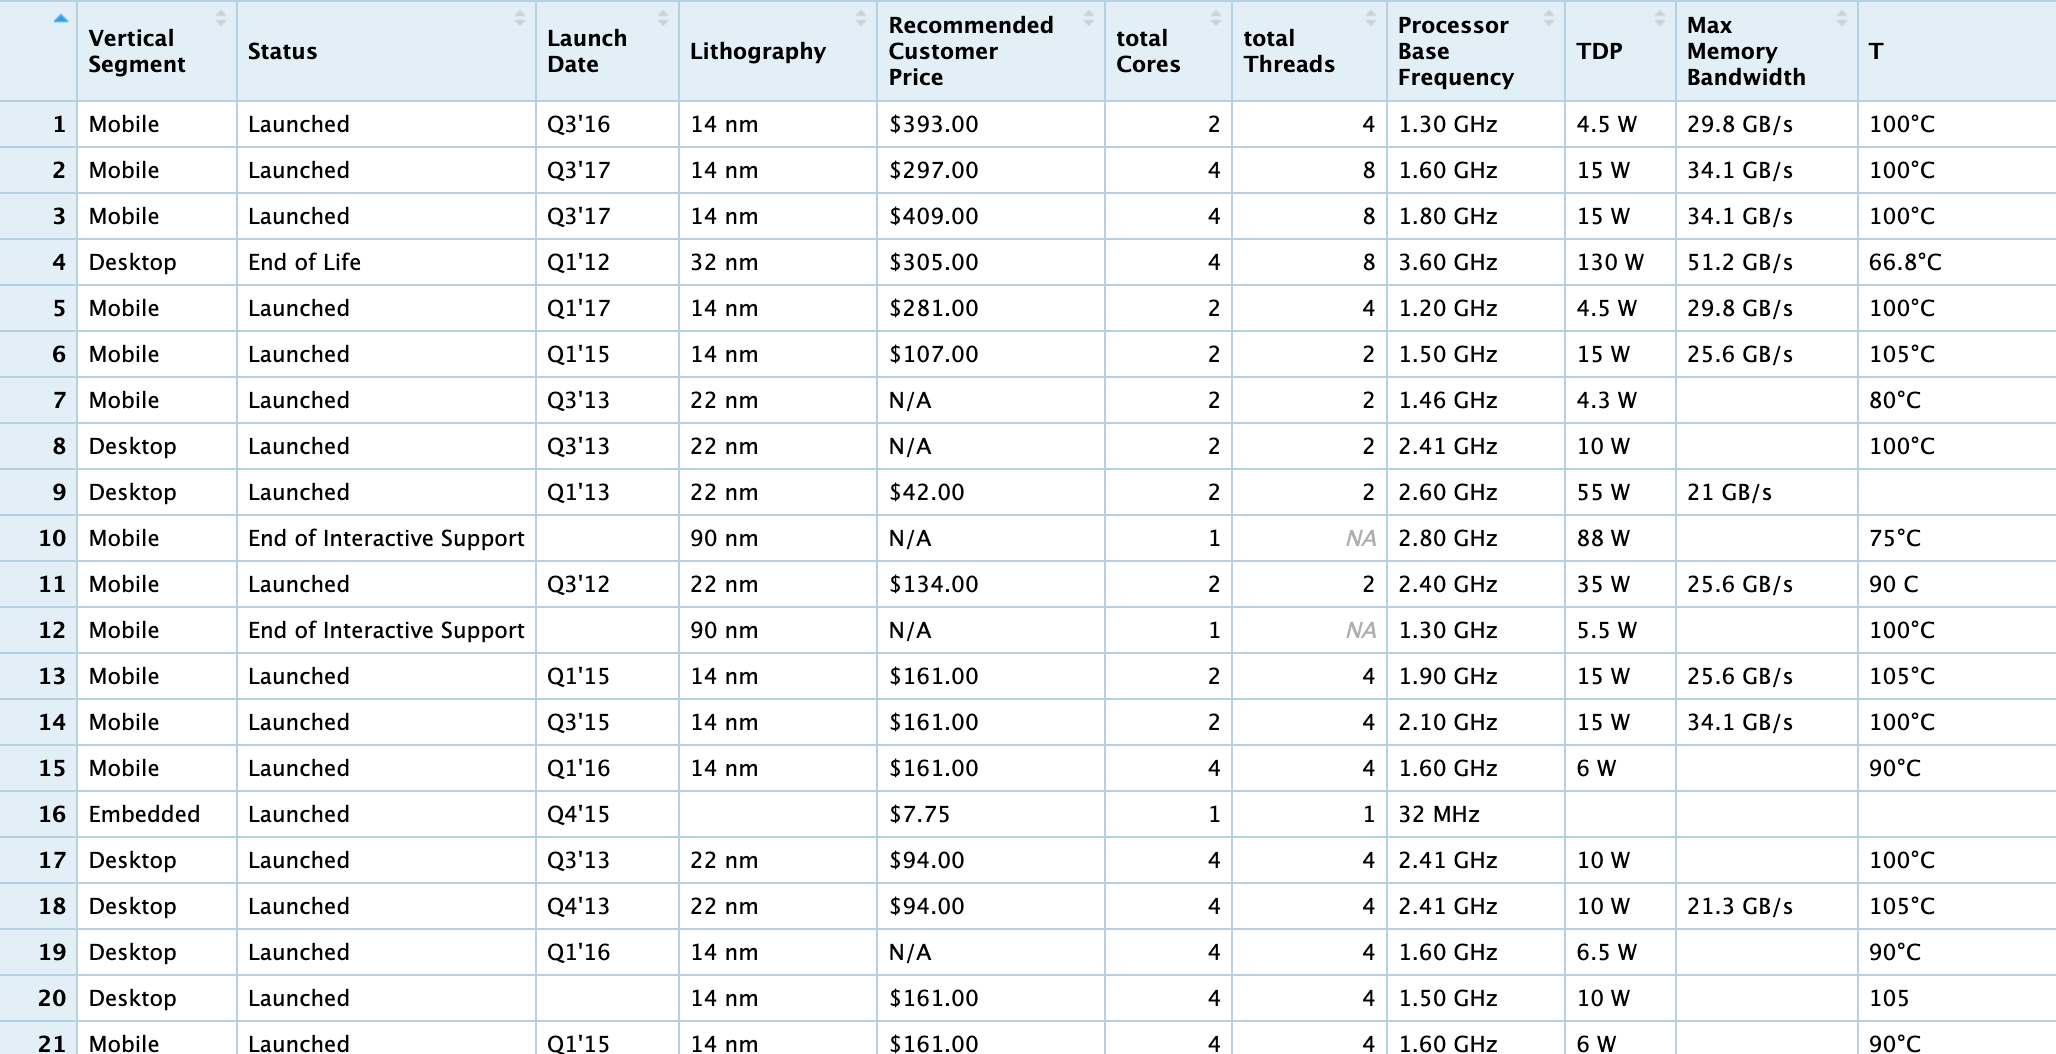
\includegraphics[max width=0.9\linewidth]{./graphics/short_data.png}
    \caption{Data before cleaning.}
\end{figure}

\subsubsection*{ldate}

\verb|market| and \verb|status| are left unchanged, since the values are straightforward. See \nameref{section:data_clarify} for further analysis.

The remaining attributes (columns) are processed as followed:

\inputcode[firstline=53,lastline=55]{R}{rcode/cleaning.r}

Our goal is to transform raw, non-standard string representation of year-quarter into \verb|zoo|'s standard representation. 
The function \mintinline{R}{as.yearqtr} takes a column and a format string as parameters. The format string is represented 
as: \mintinline{R}{"Q%q'%y"}, in which two flags \mintinline{R}{"%q"}, \mintinline{R}{"%y"} stands for quarter and year, respectively.
The format string hints the function to know the positions of quarter and year in our raw string.

\subsubsection*{litho}

\inputcode[firstline=62,lastline=64]{R}{rcode/cleaning.r}

Our goal is to cut out \verb|"nm"|, since every entry is recorded in nanometers anyway. \mintinline{R}{gsub} helps to replace a pattern 
of a string with another string. In this case, we replace any occurence of \verb|"nm"| with an empty string, and then cast the remaining 
value to numeric type. Notice that the pattern could be regular expression as well, this will be used intensively in the following cleaning
process.

\subsubsection*{rprice}

\inputcode[firstline=73,lastline=81]{R}{rcode/cleaning.r}

\textbf{HEY VIET TUNG WRITE THIS FOR ME THANK YOU!}
% YOU SHOULD EMBED THE BELOW LINE SOMEWHERE IN YOUR EXPLAINATION.
but the pattern is a regular expression (regex). Please refer to \nameref{section:appendix:regex}
for further information.

\subsubsection*{bfreq}

\inputcode[firstline=89,lastline=94]{R}{rcode/cleaning.r}

Our goal is to cut out \verb|"GHz"| and \verb|"MHz"| from the string, and convert all \verb|"MHz"| values into \verb|"GHz"|. Heuristically,
we observed that any value greater than 10 must be \verb|MHz|, so we can transform every value like that will be multiply by 0.001 to get 
the according \verb|MHz| value. \mintinline{R}{gsub} is used like as above. This time, that regex is used to match any substring that is 
\verb|GHz| OR \verb|MHz|. Then, we multiply with the 0.001 any number greater than 10, and store it back to the dataframe. Notice that the
\mintinline{R}{NA} values must be truncated first, as it is necessary to ensure dataframe subscripting to work.

\subsubsection*{tdp}

\inputcode[firstline=100,lastline=102]{R}{rcode/cleaning.r}

Our goal is to cut out \verb|"W"| from the string. The approach is similiar to the above.

\subsubsection*{memband}

\inputcode[firstline=108,lastline=110]{R}{rcode/cleaning.r}

Our goal is to cut out \verb|"GB/s"| from the string. The approach is similiar to the above.

\subsubsection*{temp}

\inputcode[firstline=124,lastline=133]{R}{rcode/cleaning.r}

Our goal is to only match the numeric values, then, take the maximum among those, since we are only interested in the maximum temperature.
This attribute's data are very varying in forms and the pattern we want is difficult if only a simple regular expression is used to match.
Our approach is can be described as follows:

\begin{itemize}
    \item First, we attempt to match every decimal numbers possible, including the irrelevant number. The rest are replaced with commas \verb|","|.
    
    The result of this process will create a string of numbers separated by commas. By doing this, the numbers are well isolated for our purpose.

    \item Second, we split these numbers and form a vector of them. This can be done through \mintinline{R}{strsplit} function. Notice that our numbers
    are still in string format.

    \item Third, we cast all these strings to numeric and push them into a vector of values using \mintinline{R}{unlist} and \mintinline{R}{lapply}
    
    \item Fourth, we find the maximum among all these values. Invalid numbers will automatically become \(-\infty\), and will be further treated as \mintinline{R}{NA}.

\end{itemize}

Notice that, we must loop through each row of the list to accomplish the above procedure.

Finally, the program produces \verb|cpu-clean.csv| as a cleaned data, ready for further exploitation in the later sections. This section uses a lot of regular expression
to match the desired strings, please refer to \nameref{section:appendix:regex} for more details.

\begin{figure}[H]
    \centering
    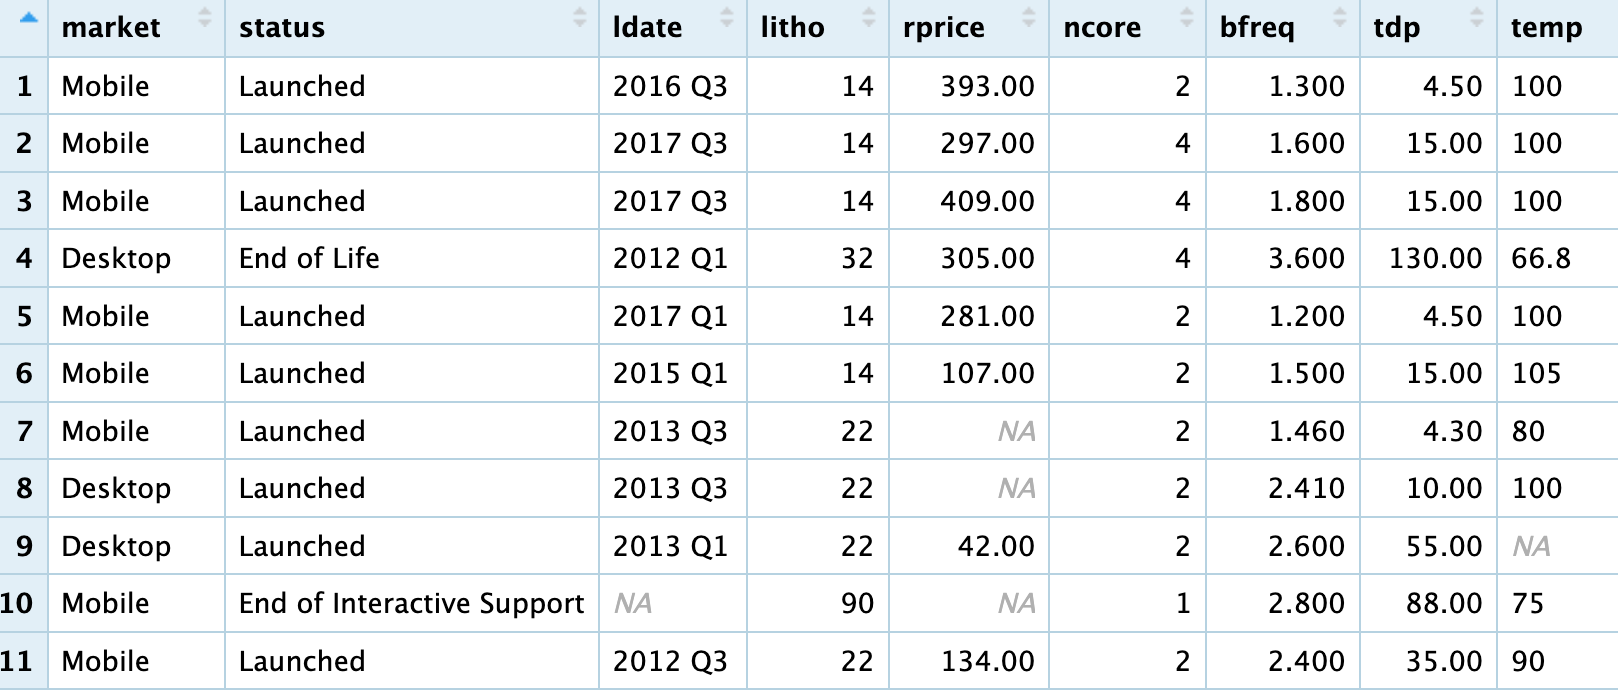
\includegraphics[max width=0.9\linewidth]{./graphics/cleaned_data.png}
    \caption{Data after cleaning.}
\end{figure}

% END OF DATA CLEANING
%
%   Data Clarification
%       - Plots...
%   
\clearpage
\section{Data clarification}
\label{section:data_clarify}

This section provides several visualizations to highlight the big pictures of our dataset, and it would
focus mostly on the behaviour of each variable as independent individuals, rather than the interaction 
between them, which we will focus in much details in \textbf{Section \ref{section:data_analysis}}.

\subsection{Categorical attributes}

\begin{figure}[H]
    \centering
    \begin{subfigure}[b]{0.49\textwidth}
        \centering
        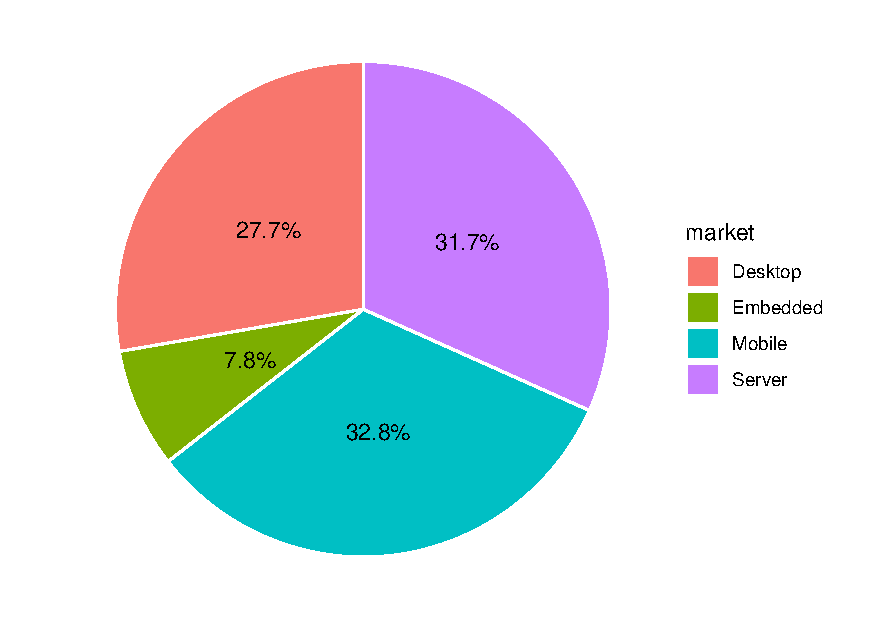
\includegraphics[width=\textwidth]{./graphics/pie_market.pdf}
        \caption{Pie of market share}
    \end{subfigure}
    \hfill
    \begin{subfigure}[b]{0.49\textwidth}
        \centering
        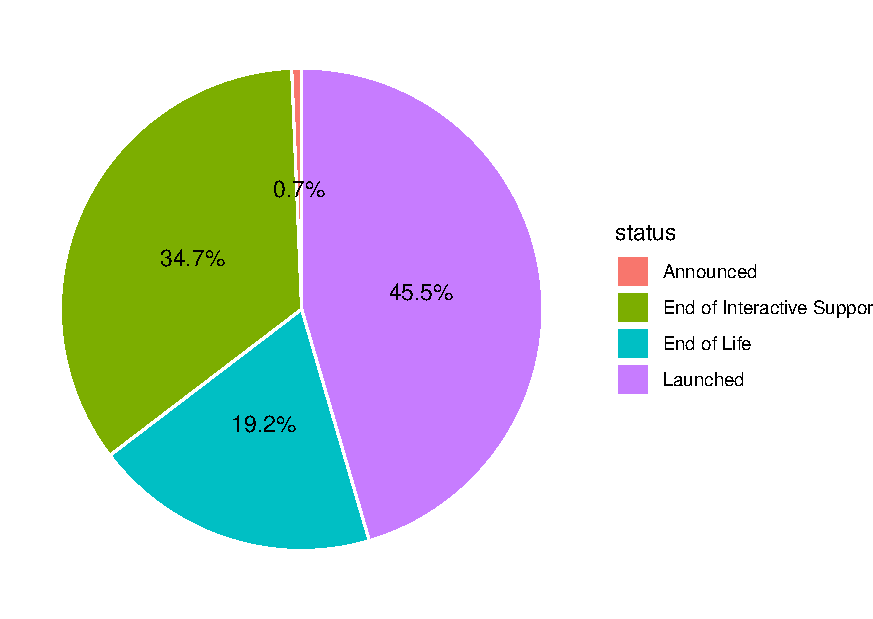
\includegraphics[width=\textwidth]{./graphics/pie_status.pdf}
        \caption{Pie of status}
    \end{subfigure}
    \caption{Pies of categorical attributes}
    \label{fig:pie_category}
\end{figure}

\inputcode[firstline=59,lastline=73]{R}{rcode/clarification.rmd}

\textbf{[Figure \ref{fig:pie_category}]} Two obvious categorical attributes of our data are \textit{Market} and \textit{Status}.
\begin{itemize}
    \item In \textit{Market} attribute, three primary shares of market are Desktop, Server and Mobile. Embedded constitues a very small
    proportion.
    \item In \textit{Status} attribute, most of them are Launched, End of Life or End of interactive support. A tiny amount of Announce
    contributes modestly to total amount of CPU's model by provider Intel.
\end{itemize}

In terms of the code we used to plot two above pies. Each line is self-explanatory. Since two pies have different configurations, and would be
verbose to explain everything here, we leave the detailed implementation in \verb|rcode/clarification.rmd|. A few things to note are:
\begin{itemize}
    \item \verb|data_percentages| is a data-frame containing three properties: \verb|market|, \verb|value| and \verb|percent|.
    Note that, we use variable \verb|market| two times: one for plotting market-pie and one for plotting status-pie. This is just for ease
    of use and avoid repeating the code. It should not be taken seriously (the same name for two different things could be confusing).
    \item \verb|market| are the levels of \verb|market|-attribute (or \verb|status|-attribute)
    \item \verb|value| is the vector of frequencies of each \verb|market| (or \verb|status|)
    \item \verb|percent| is the vector percentages (computed by dividing the frequency by total and multiply by $100$)
\end{itemize}





\subsection{Continuous attributes}

\begin{figure}[H]
    \centering
    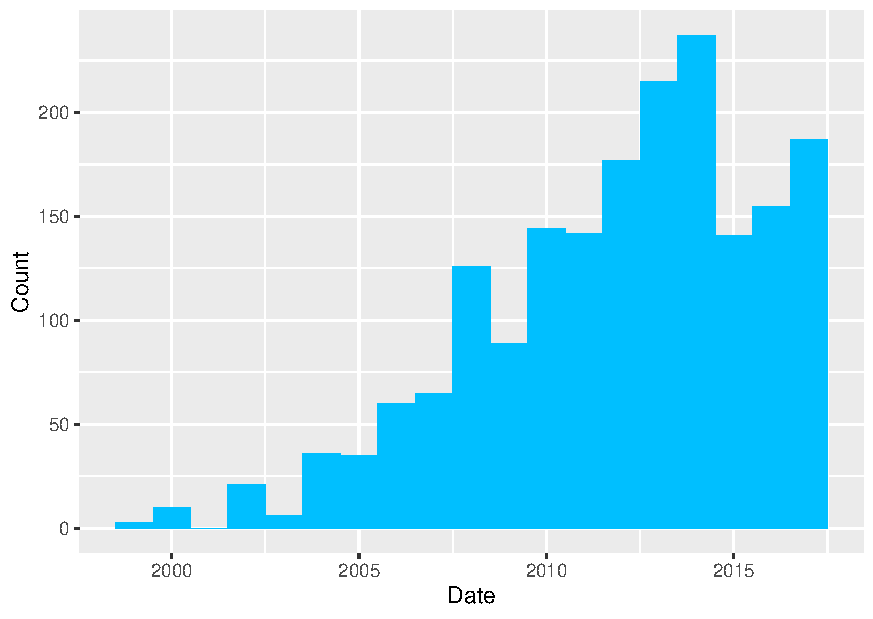
\includegraphics[width=0.5\textwidth]{./graphics/hist_ldate.pdf}
    \caption{Histogram of launch date}
    \label{fig:hist_ldate}
\end{figure}

\inputcode[firstline=78,lastline=80]{R}{rcode/clarification.rmd}

\textbf{[Figure \ref{fig:hist_ldate}]} The \textit{Launch date} histogram shown that most of Intel's CPUs are launched recently, 
with two notable peaks at 2014 and 2017. This would affect tremendously to the bias of the data since some variables are dependent 
on \textit{Launch date}, making the prediction models (\textbf{Section \ref{section:data_analysis}}) weight the recent CPUs heavily,
instead of old, legacy CPUs which are also neccessary to capture a fair pattern over the time.






\begin{figure}[H]
    \centering
    \begin{subfigure}[b]{0.49\textwidth}
        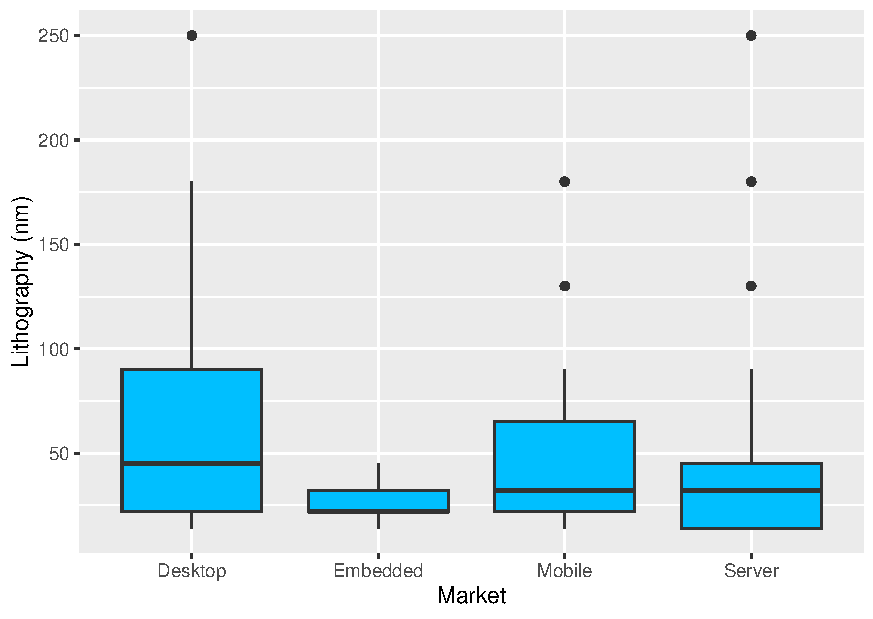
\includegraphics[width=\textwidth]{./graphics/box_litho.pdf}
        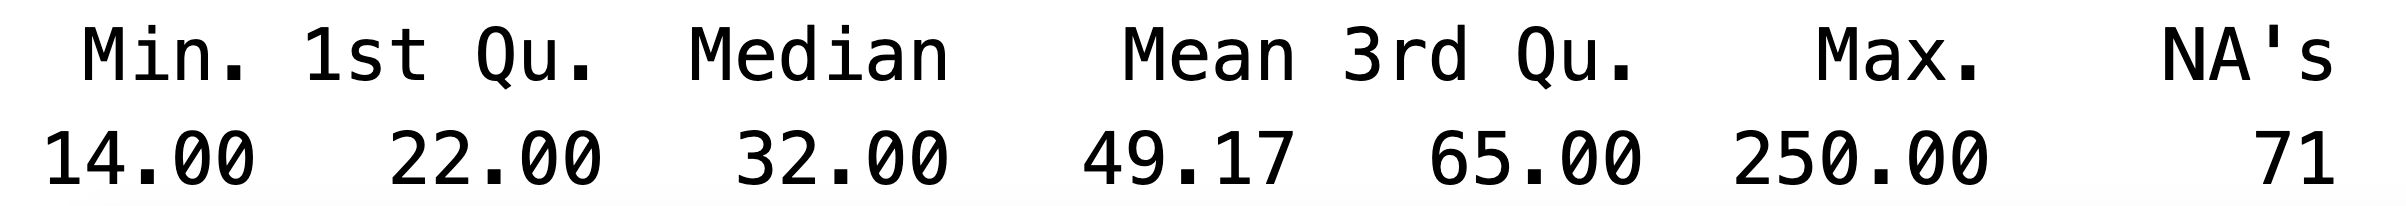
\includegraphics[width=\textwidth]{./graphics/sum_litho.png}
        \caption{Box plots and Summary of Lithography}
        \label{fig:box_litho}
    \end{subfigure}
    \hfill
    \begin{subfigure}[b]{0.49\textwidth}
        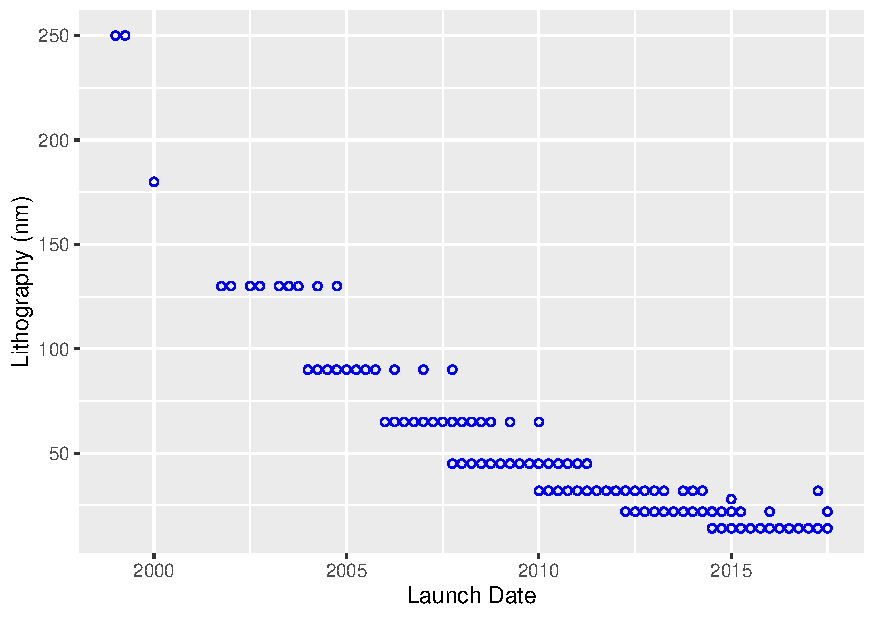
\includegraphics[width=\textwidth]{./graphics/scatter_litho.pdf}
        \caption{Plot of lithography over time.}
        \label{fig:scatter_litho}
    \end{subfigure}
    \caption{Lithography plots}
\end{figure}

\inputcode[firstline=85,lastline=89]{R}{rcode/clarification.rmd}

\inputcode[firstline=94,lastline=96]{R}{rcode/clarification.rmd}

\textbf{[Figure \ref{fig:box_litho}]} The box plot of \textit{Lithography} (chip printing technique) demonstrates interesting characteristics:
\begin{itemize}
    \item There was a large variance in the types of Lithography designed in Intel's Desktop processors, a smaller, but significant variance of 
    Mobile and Server are also observed. Embedded is less diverse, however, and also concentrates mostly on small \textit{Lithography} printings.

    \item The mean of \textit{Lithography}, in whatever market, is also approximately the same. That number might represents the most suitable 
    printing technique that is widely used among Intel's CPUs.
\end{itemize}

Overall, the most common \textit{Lithography} is $32 nm$. The best printing technique possible was $14 nm$ and the worst was $250 nm$. That large
number might come from old, legacy processors which were not designed with recent innovations in the Chip industry.

\textbf{[Figure \ref{fig:scatter_litho}]} The scatter plot of \textit{Lithography} with respect to \textit{Launch date} shown that the lithography
is getting smaller over time, and they are categorized into specific time intervals. The fact the \textit{Lithography} spans the distribution over
an interval of time instead of condensed into a specific quarter like \textit{Launch date} make it more powerful than \textit{Launch date}. In our
models, we always use \textit{Lithography} instead of \textit{Launch date}. This fact will be visualized with numbers later to make this argument 
more convincing.







\begin{figure}[H]
    \centering
    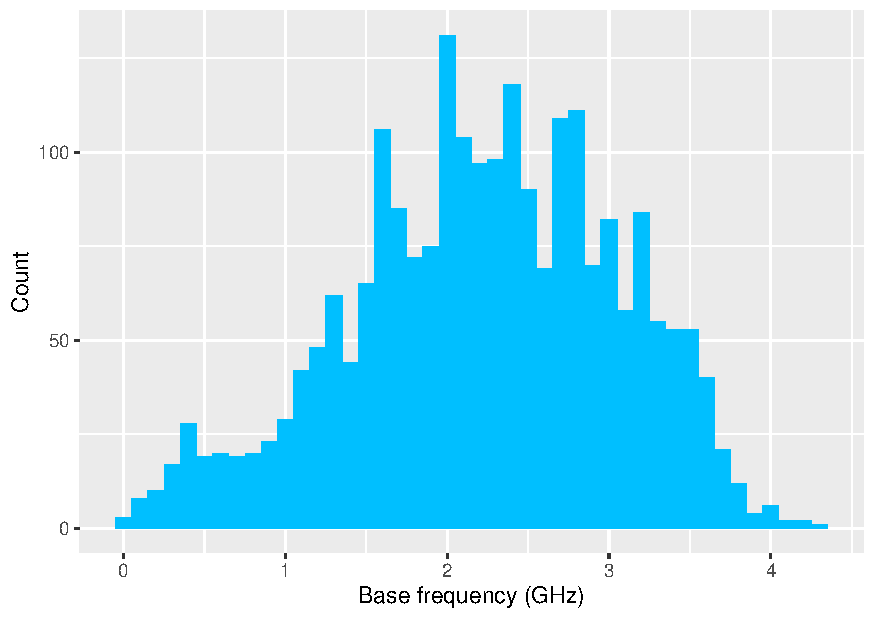
\includegraphics[width=0.5\textwidth]{./graphics/hist_bfreq.pdf}
    \caption{Histogram of Base Frequency}
    \label{fig:hist_bfreq}
\end{figure}

\inputcode[firstline=108,lastline=110]{R}{rcode/clarification.rmd}

\textbf{[Figure \ref{fig:hist_bfreq}]} The most significant trend that could be observed in the \textit{Base frequency} histogram is its "normality".
It can be seen that, the shape of \textit{Base frequency} disribution is convincingly a bell, and most \textit{Base frequency} concentrates around
the mean (around $2.3$ GHz). This is expected since high \textit{Base frequency} can influence the amound of heat a CPU produces, and there are always
trade-offs between performance and heat. This relationship (between heat and performance) will be visualized in \textbf{Section \ref{section:data_analysis}}.






\begin{figure}[H]
    \centering
    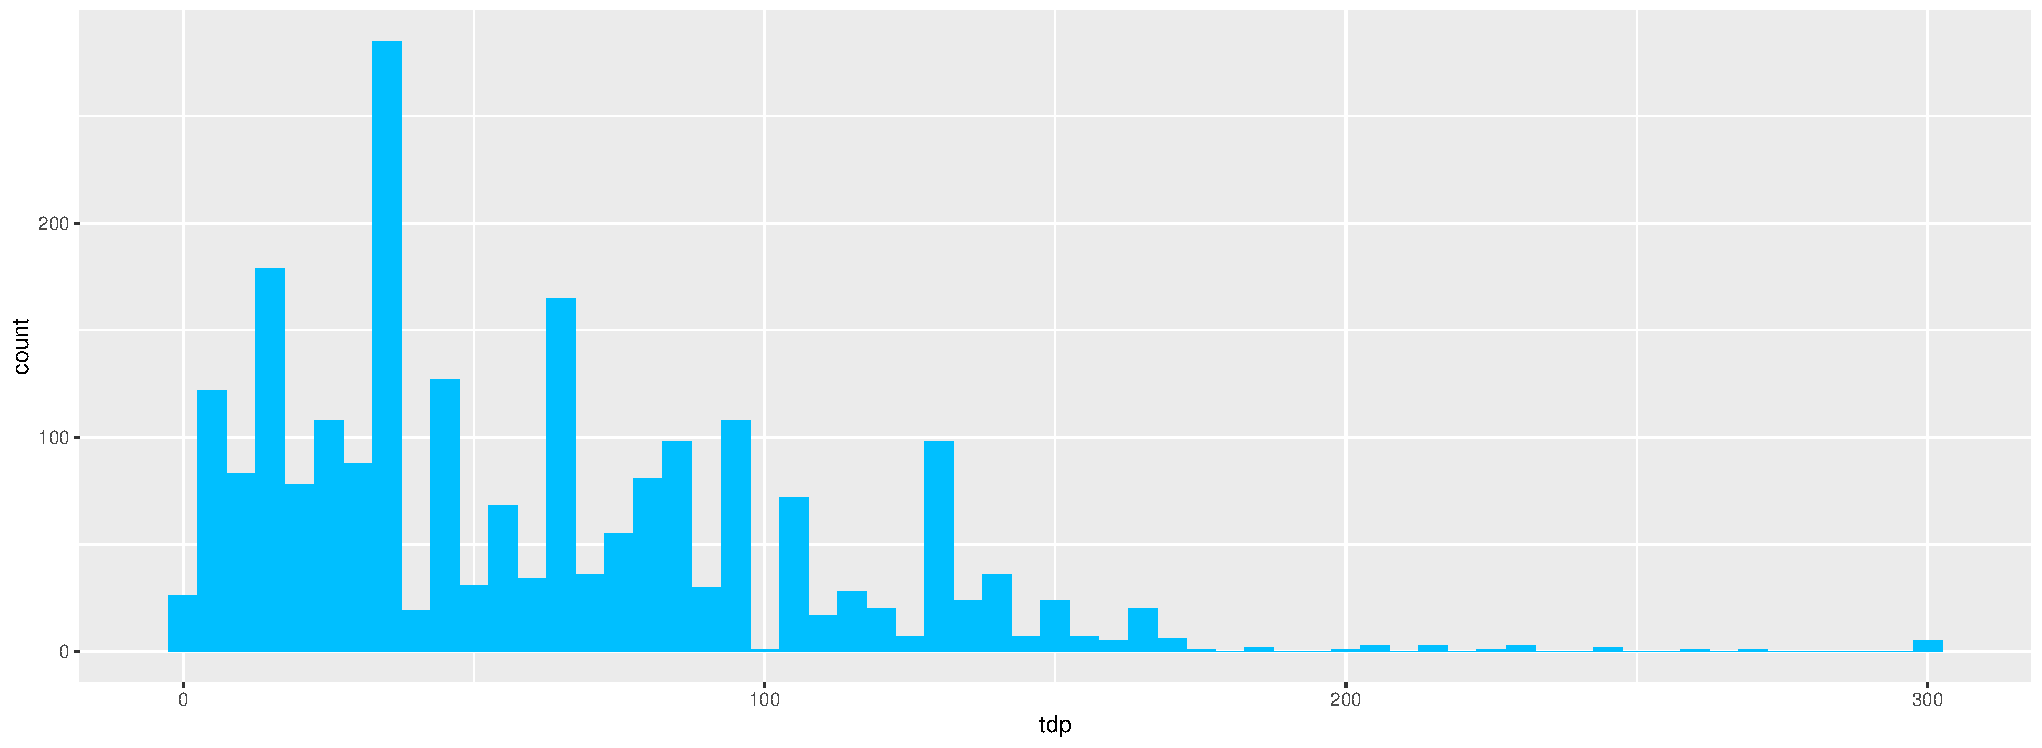
\includegraphics[width=0.5\textwidth]{./graphics/hist_tdp.pdf}
    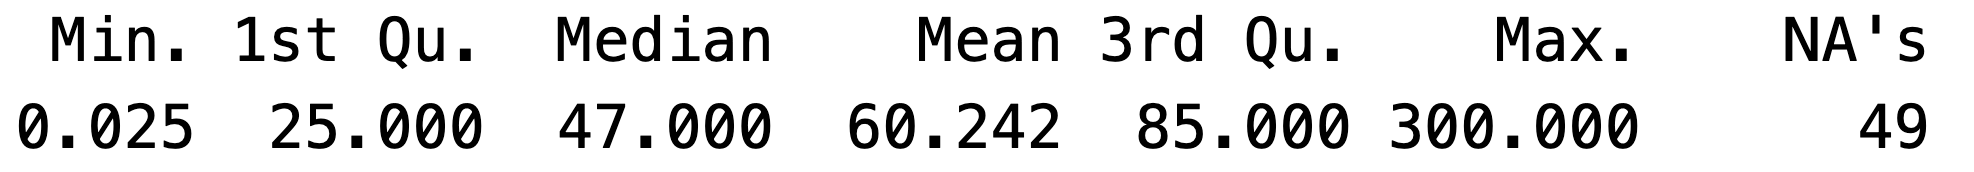
\includegraphics[width=0.5\textwidth]{./graphics/sum_tdp.png}
    \caption{Box plots and Summary of Thermal Design Power}
    \label{fig:hist_tdp}
\end{figure}

\inputcode[firstline=115,lastline=119]{R}{rcode/clarification.rmd}

\textbf{[Figure \ref{fig:hist_tdp}]} \textit{Thermal design power} is the of main interest in our topic. We can see that, the distribution of \verb|TDP| varies
wildly, from 0W to 300W. However, the occurences of values $\ge 150$W is rare (we can see the 75\%-quantile is at 85W), indicating that we can treat these values 
as outliners and remove them before carrying further analysis.
%
%   Data Analysis
%       - ANOVA and Regression and stuff.
%   
\clearpage
\section{Data analysis}
\label{section:data_analysis}









\subsection{Analysis of Variance (ANOVA)}

In this section, we analyze the relationships between variables, namely \verb|bfreq| with respect to \verb|litho| and \verb|ncore|.

There are interesting facts about the above attributes:
\begin{itemize}
    \item \verb|bfreq| is a very good representative for CPU's performance, so we will explore
    how other factors contribute to the performance of the CPU.
    \item \verb|litho| represents well for the distinction of each period, in fact, it is
    a better representation for \verb|ldate|. Refer to \textbf{[Figure \ref{fig:scatter_litho}]} we provided in the last section,
    with bare eyes, we can see `litho` is associated with the launch-date very well, and
    it is decreasing over time. What makes it better than \verb|ldate| is that \verb|litho| spans
    over a period of time, and not fixed to a specific year-quarter. One more advantage
    is that, some records do not have launch dates, but they have lithography instead, so using
    it is better to gain more data. We would like to see the impact of decreasing lithography
    on the performance of the CPU.
    \item \verb|ncore| is the driving factor of modern computing, which helps computer utilizing 
    the power of parallelization. This is considered to be a work-around for the approaching lower limit Lithography of 1.5 nanometers
    \cite{2nm-barrier}. On the other hand, more cores also means more cost 
    for a CPU to be manufactured. Because of that, analyzing the number of cores with respect to its perform is neccessary to decide
    whether it is worthy to invest a lot of money produce cores, and whether increasing no. cores impact negatively to the base frequency.
\end{itemize}

Because of that, we chose to analyze them to get a good insight over our CPU dataset.

Refer to \textbf{Figure \ref{fig:box_bfreq_wrt_ncore_litho}}, we can observe that the means of \textit{Base frequency} 
of each \textit{Lithography} were approximately the same when \verb|ncore = 4|, while they were more fluctuated for \verb|ncore = 2|.
From that, we have the following hypotheses:
\begin{enumerate}
    \item For \verb|ncore = 4|, the \textit{Base frequencies} are the same among all groups of \textit{Lithography}.
    \item 
    \item adkgjakdsg
    \item adgkajdhg
\end{enumerate}

\subsubsection{Kruskal-Wallis One-way ANOVA}

\subsubsection{Rank-based Two-way ANOVA}

\subsubsection{Conclusion}





\subsection{Regression models}
%
%   Conclusion
%
%   What did we find?
%   
\clearpage
\section{Conclusion}
\section{Appendix}
\label{section:appendix}

\label{section:appendix:regex}
Regular expression appendix











 \bibliographystyle{plain}
 \bibliography{refs}
\nocite{*}

\end{document}
